%% LaTeX-Beamer template for KIT design
%% by Erik Burger, Christian Hammer
%% title picture by Klaus Krogmann
%%
%% version 2.1
%%
%% mostly compatible to KIT corporate design v2.0
%% http://intranet.kit.edu/gestaltungsrichtlinien.php
%%
%% Problems, bugs and comments to
%% burger@kit.edu

\documentclass[18pt]{beamer}

%% SLIDE FORMAT

% use 'beamerthemekit' for standard 4:3 ratio
% for widescreen slides (16:9), use 'beamerthemekitwide'

\usepackage{templates/beamerthemekit}
% \usepackage{templates/beamerthemekitwide}

%% TITLE PICTURE

% if a custom picture is to be used on the title page, copy it into the 'logos'
% directory, in the line below, replace 'mypicture' with the 
% filename (without extension) and uncomment the following line
% (picture proportions: 63 : 20 for standard, 169 : 40 for wide
% *.eps format if you use latex+dvips+ps2pdf, 
% *.jpg/*.png/*.pdf if you use pdflatex)

\titleimage{title}

%% TITLE LOGO

% for a custom logo on the front page, copy your file into the 'logos'
% directory, insert the filename in the line below and uncomment it

%\titlelogo{mylogo}

% (*.eps format if you use latex+dvips+ps2pdf,
% *.jpg/*.png/*.pdf if you use pdflatex)

%% TikZ INTEGRATION

% use these packages for PCM symbols and UML classes
% \usepackage{templates/tikzkit}
% \usepackage{templates/tikzuml}

% the presentation starts here

\title[Specification presentation]{Dynamic scheduler for scientific simulations}
\subtitle{Final presentation}
\author{Kai Bittner, Ard Kastrati, Fabio Broghammer, Jan Ellmers, David Krenz, Benjamin-Philip Roth}

\institute{Steinbuch Centre for Computing - SCC}

% Bibliography

\usepackage[citestyle=authoryear,bibstyle=numeric,hyperref,backend=biber]{biblatex}
\addbibresource{templates/example.bib}
\bibhang1em
\usepackage{graphicx}
\usepackage{tikz}
\usetikzlibrary{shapes}
\begin{document}

% change the following line to "ngerman" for German style date and logos
\selectlanguage{english}

%title page
\begin{frame}
\titlepage
\end{frame}

%table of contents
\begin{frame}{Outline}
\tableofcontents
\end{frame}


\section{Overview}
\begin{frame}{Overview}

\centerline{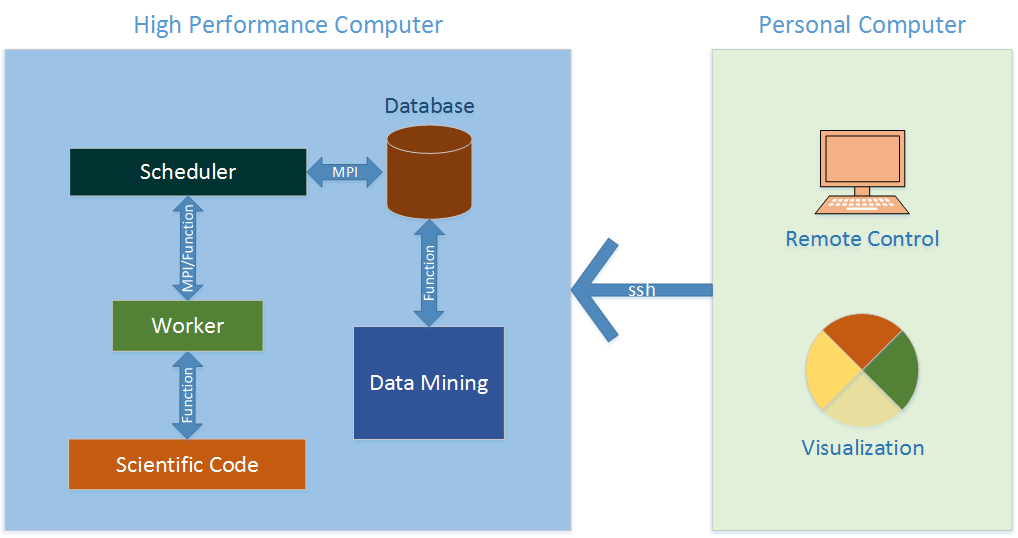
\includegraphics[scale=0.43]{images/overview}}
\end{frame}


	\begin{frame}{Master-Worker}
		\centerline{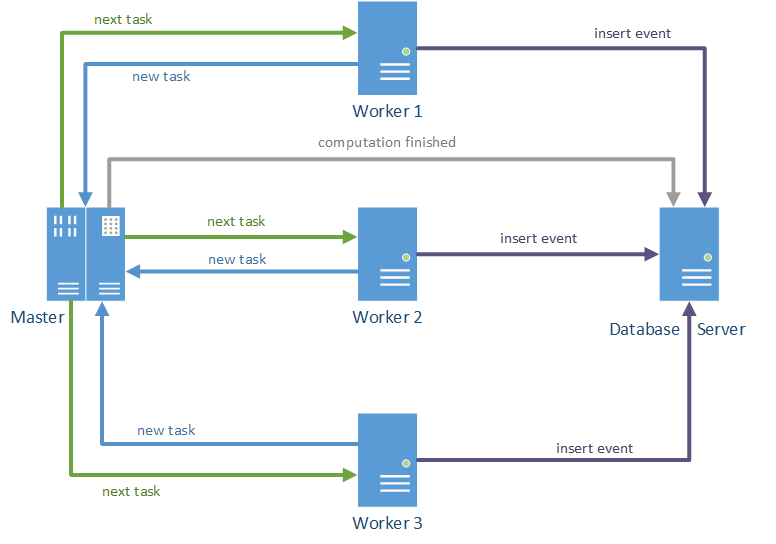
\includegraphics[scale=0.5]{images/master}}
	\end{frame}
	\begin{frame}{Task Stealing}
		\centerline{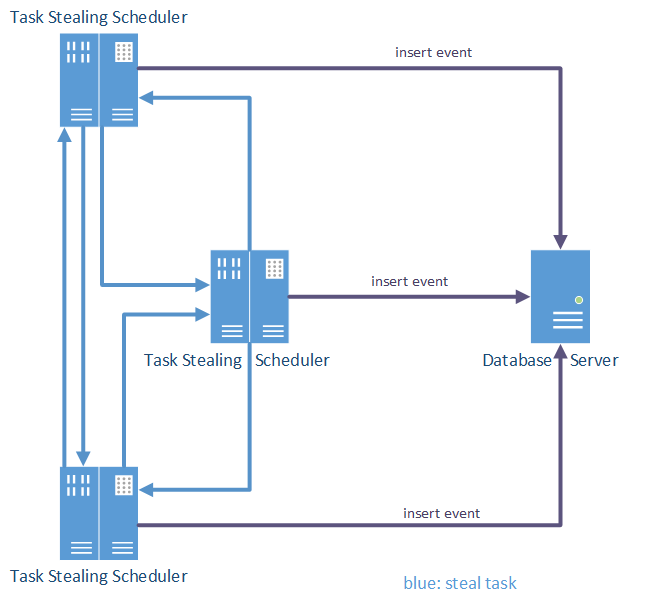
\includegraphics[scale=0.5]{images/taskstealing}}
	\end{frame}

	\begin{frame}{Scheduling Strategies}
	\begin{minipage}[]{.7\textwidth}%
			\begin{itemize}
		\item<2-> Non-statistical
		\begin{itemize}
			\item<3-> First In-First Out (FIFO)
			\item<4-> Last In-Fist Out (LIFO)
		\end{itemize}
		\item<5-> Statistical
		\begin{itemize}
			\item<6-> Shortest Job First (SJF)
			\item<7-> Longest Job First (LJF)
		\end{itemize}
		\item<8-> Standardized interface 
			\begin{itemize}
				\item<9-> simple to include new strategies
			\end{itemize}					
		\end{itemize}
\end{minipage}%
\begin{minipage}[]{.3\textwidth}%
  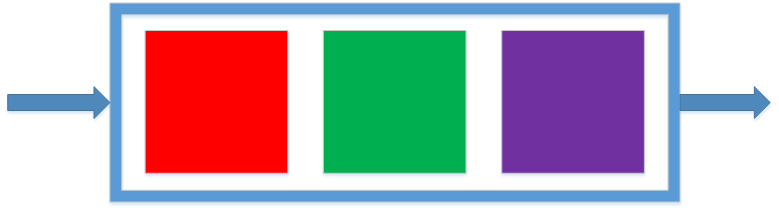
\includegraphics[width=\textwidth]{images/fifo}%
\end{minipage}		
		
	\end{frame}
	\begin{frame}{Master-Worker vs. Task Stealing}
		\begin{itemize}
			\item<2-> Master-Worker
				\begin{itemize}
					\item<3-> fast standard c++ implementation
					\item<4-> dynamic size
					\item<5-> easy to switch between scheduling strategies at runtime	
				\end{itemize}
			
			\item<6-> Task stealing
					\begin{itemize}
						\item<7-> custom implementation inside a MPI-Window
					\end{itemize}
			
		\end{itemize}
	\end{frame}


	\begin{frame}{Metadata}
	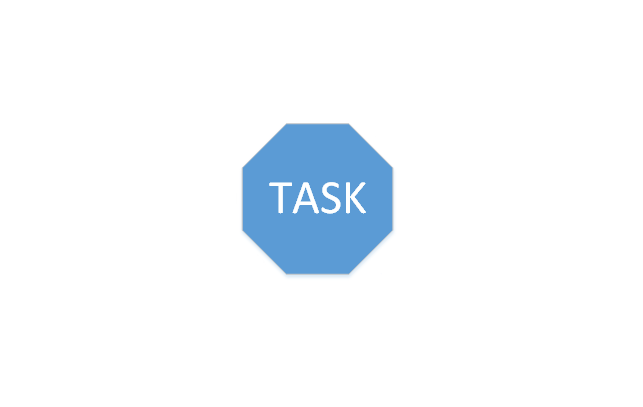
\includegraphics[width=1.0\textwidth]{images/Task/zeichnungstep5.png}
	\end{frame}
	
	\begin{frame}{Metadata}
	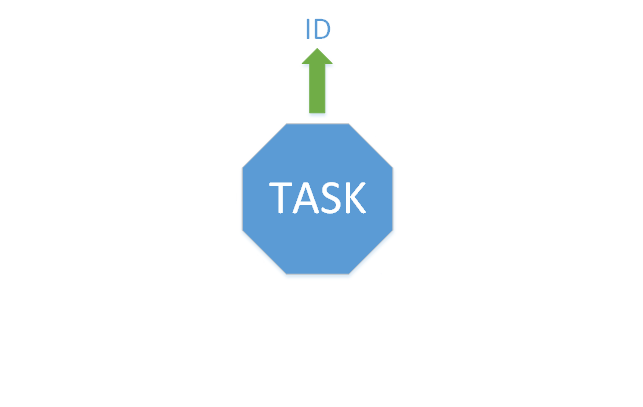
\includegraphics[width=1.0\textwidth]{images/Task/zeichnungstep4.png}
	\end{frame}
	
	\begin{frame}{Metadata}
	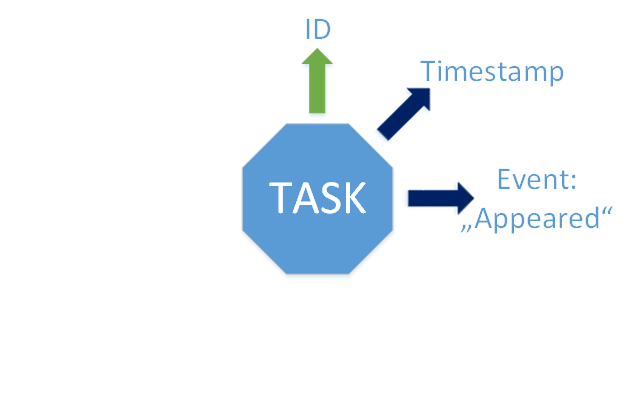
\includegraphics[width=1.0\textwidth]{images/Task/zeichnungstep3.png}
	\end{frame}
	
	\begin{frame}{Metadata}
	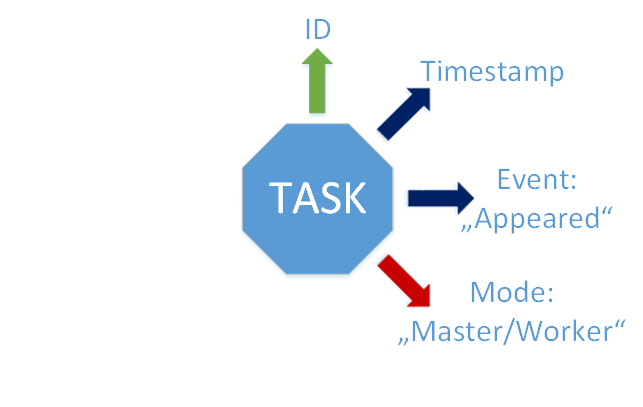
\includegraphics[width=1.0\textwidth]{images/Task/zeichnungstep2.png}
	\end{frame}
	
	\begin{frame}{Metadata}
	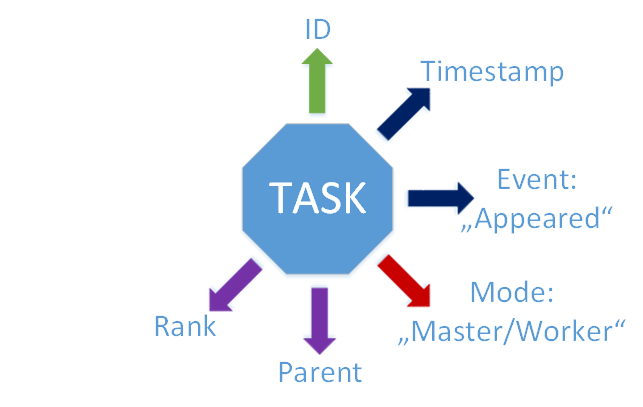
\includegraphics[width=1.0\textwidth]{images/Task/zeichnungstep1.png}
	\end{frame}
	
	\begin{frame}{Metadata}
	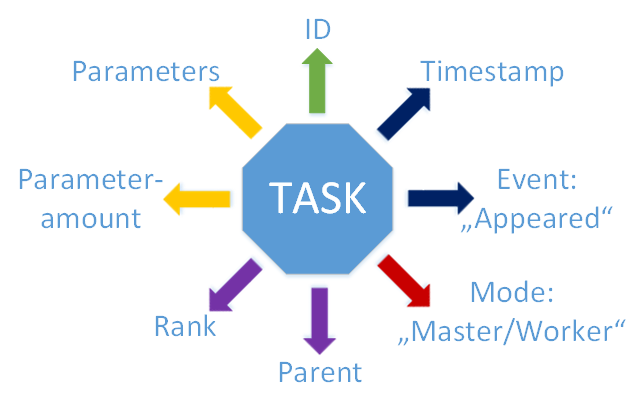
\includegraphics[width=1.0\textwidth]{images/Task/Zeichnung1.png}
	\end{frame}
	
	\begin{frame}{Metadata}
	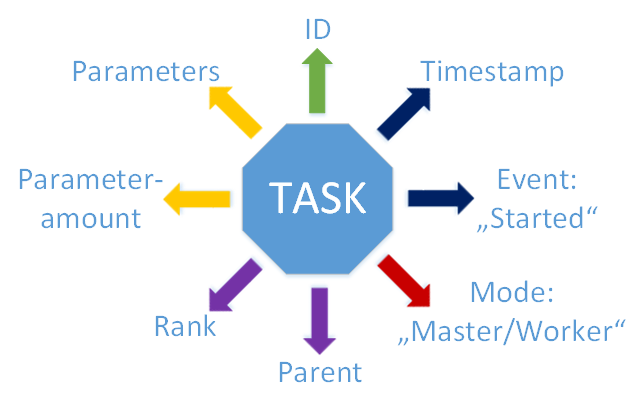
\includegraphics[width=1.0\textwidth]{images/Task/Zeichnung2.png}
	\end{frame}
	
	\begin{frame}{Metadata}
	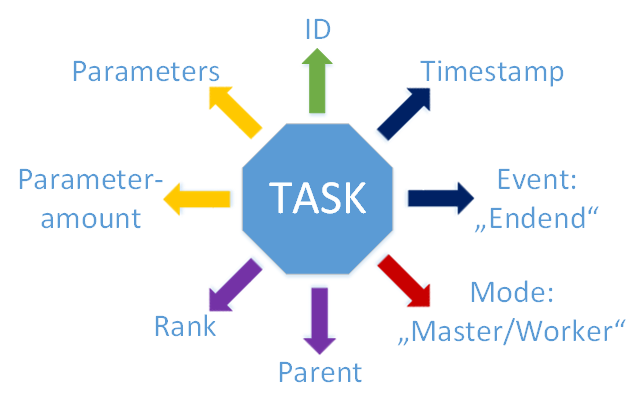
\includegraphics[width=1.0\textwidth]{images/Task/Zeichnung3.png}
	\end{frame}
	
	\begin{frame}{Metadata}
	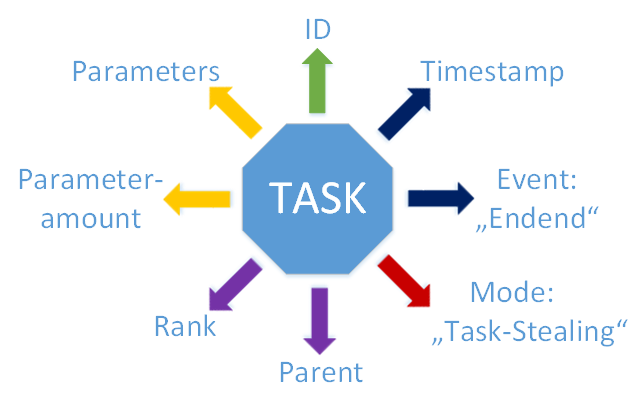
\includegraphics[width=1.0\textwidth]{images/Zeichnungedited.png}
	\end{frame}
	
	\begin{frame}{Structure}
		\begin{minipage}[]{.5\textwidth}%
		\begin{itemize}
		\item<2->{} {Data stored in 2 separate files}
		\item<3->{} {Bookkeeping: listed data of previous slide}
		\item<4->{} {Statistics: parameters and runtime of a task}
		\item<5->{} {\textbf{Additionally: }files are accessible for visualizer}
		\end{itemize}
		\end{minipage}
		\begin{minipage}[]{.45\textwidth}%
		\begin{figure}[h]
		\flushright  % rechtsbuendig
		\vspace{-\ht\strutbox}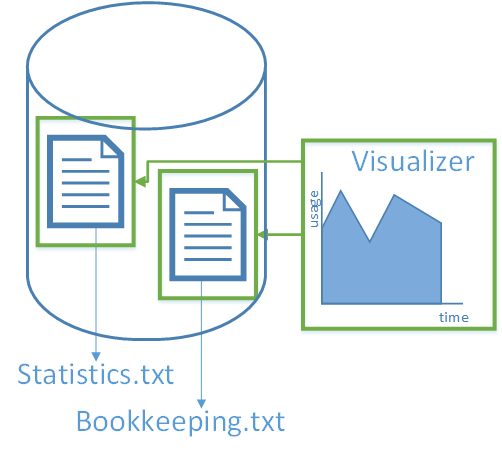
\includegraphics[width=\textwidth]{images/data.png}
		\end{figure}
		\end{minipage}
	\end{frame}
%\subsubsection{handling}
	\begin{frame}{Database Handler}
	
	\begin{minipage}[]{.5\textwidth}%
	\begin{itemize}
		\item<2->{} {Provide methods for data parsing}
		\item<3->{} {Transmit data}
	\end{itemize}
	\end{minipage}	
	\begin{minipage}[]{.25\textwidth}%
	\vspace{-\ht\strutbox}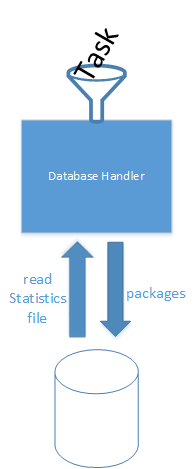
\includegraphics[width=\textwidth]{images/zeichnunghandler.png}
	\end{minipage}%
	
	\end{frame}
	
	\begin{frame}{Database Server}
	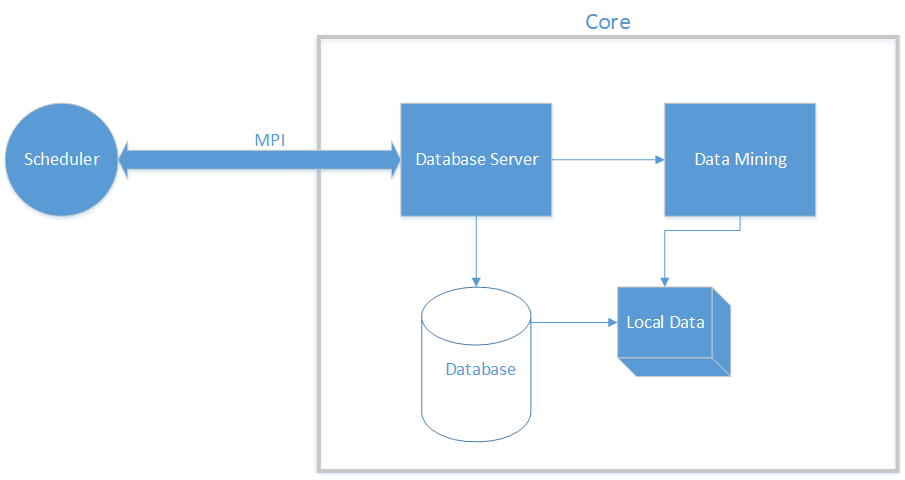
\includegraphics[width=1.0\textwidth]{images/databaseserver.png}
	\end{frame}
	
	\begin{frame}{Connection to Data Mining}
	\begin{center}
	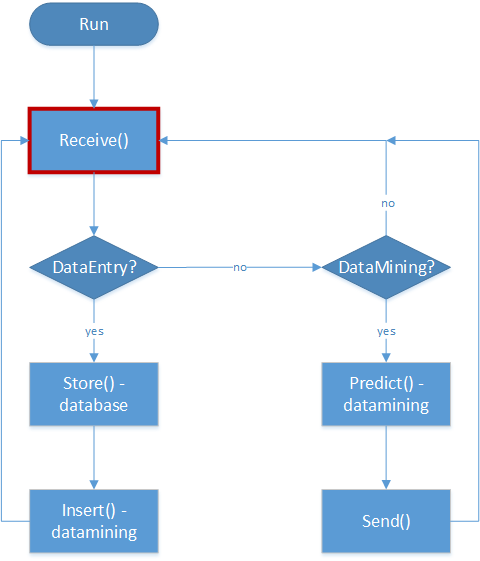
\includegraphics[height=0.64\textwidth, width=0.6\textwidth]{images/datamining_flow0.png}
	\end{center}
	\end{frame}
	
	\begin{frame}{Connection to Data Mining}
		\begin{center}
	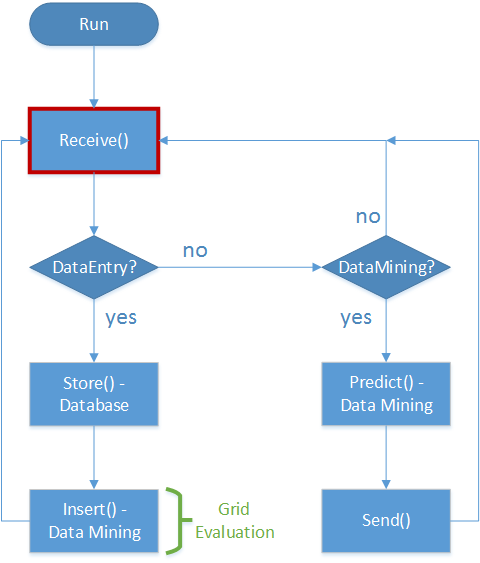
\includegraphics[height=0.64\textwidth, width=0.6\textwidth]{images/datamining_flow1.png}
	\end{center}
	\end{frame}
	
	\begin{frame}{Connection to Data Mining}
		\begin{center}
	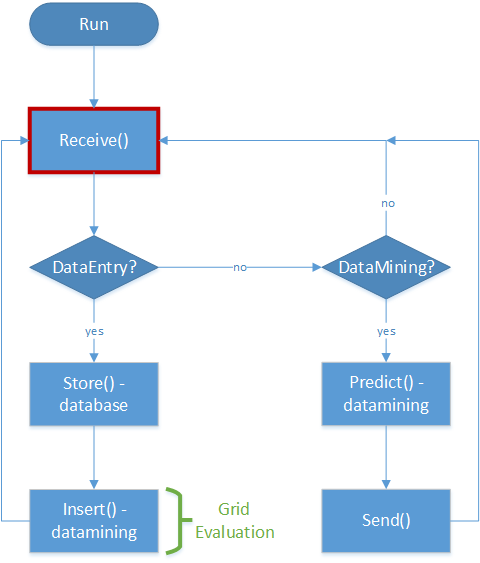
\includegraphics[height=0.64\textwidth, width=0.6\textwidth]{images/datamining_flow2.png}
	\end{center}
	\end{frame}



\begin{frame}
	\frametitle{Objectives}
		\begin{itemize}
			\item<2-> {Estimate runtime in 'constant' time}
				\begin{itemize}
					\item<3-> {Constant to the amount of tasks already executed}	
				\end{itemize}
				\item<4-> {Estimation based on variable amounts of parameters}
			\end{itemize}
\end{frame}		
		
\begin{frame} 
	\frametitle{Concepts}
		\begin{itemize}
			\item<2-> {Strong correlation between parameters and runtime of a task}
			\item<3-> {Tasks with similar parameters have similar runtime}
				\begin{itemize}
					\item<4-> {tasks with identical parameters have identical runtime}	
				\end{itemize}	
		\end{itemize}
\end{frame}


\begin{frame}
	\frametitle{Basic Design I}
	\begin{minipage}[t]{0.42\linewidth}
		\begin{itemize}
			\item<2-> {Array of 'grid points'}
				\begin{itemize}
					\item<3-> {similar to a Cartesian coordinate system}
					%\item<3->{grid points: "pointer" to 'closest' task already executed}
					%\begin{itemize}
					%	\item<4->{closest defined as 'smallest parameter differences'}	
					%\end{itemize}
				\end{itemize}	
		\end{itemize}
	\end{minipage}\hfill
	\begin{minipage}[t]{0.58\linewidth}
		\vspace{-\ht\strutbox}
	\begin{tikzpicture}[scale = 0.5]
		\draw[->, very thick] (0,0) -- (7, 0) node[right] {param 1};
		\draw[->, very thick] (0,0) -- (0, 8) node[above] {param 2};
		
		\fill (1, 2) circle (0.5mm);
		\fill (2, 2) circle (0.5mm);
		\fill (3, 2) circle (0.5mm);
		\fill (4, 2) circle (0.5mm);
		\fill (5, 2) circle (0.5mm);
	
		\fill (1, 3) circle (0.5mm);
		\fill (2, 3) circle (0.5mm);
		\fill (3, 3) circle (0.5mm);
		\fill (4, 3) circle (0.5mm);
		\fill (5, 3) circle (0.5mm);
	
		\fill (1, 4) circle (0.5mm);
		\fill (2, 4) circle (0.5mm);
		\fill (3, 4) circle (0.5mm);
		\fill (4, 4) circle (0.5mm);
		\fill (5, 4) circle (0.5mm);
		
		\fill (1, 5) circle (0.5mm);
		\fill (2, 5) circle (0.5mm);
		\fill (3, 5) circle (0.5mm);
		\fill (4, 5) circle (0.5mm);
		\fill (5, 5) circle (0.5mm);
		
		\fill (1, 6) circle (0.5mm);
		\fill (2, 6) circle (0.5mm);
		\fill (3, 6) circle (0.5mm);
		\fill (4, 6) circle (0.5mm);
		\fill (5, 6) circle (0.5mm);
		
		\begin{scope}[>= Latex]
			\draw[->, very thick] (6, 6) node[right]{grid point}  --  (5.05, 6) ;
		\end{scope}
	\end{tikzpicture}
	\end{minipage}		
\end{frame}

\begin{frame}
	\frametitle{Basic Design II}
	\begin{minipage}[t]{0.48\linewidth}
		%\begin{itemize}
		%	\item<1-> {Array of 'grid points'}
				\begin{itemize}
		%			\item<2-> {Similar to a Cartesian coordinate system}
					\item<2->{Grid points: "pointer" to 'closest' task already executed}
					\begin{itemize}
						\item<3->{closest defined as 'smallest parameter differences'}	
					\end{itemize}
				\end{itemize}	
		%\end{itemize}
	\end{minipage}\hfill
	\begin{minipage}[t]{0.48\linewidth}
		\vspace{-\ht\strutbox}
	\begin{tikzpicture}[scale = 0.8]
	%\fill[white] (-2, 6) circle (0.01);
	
		\fill (1, 2) circle (0.5mm);
		\fill (5, 2) circle (0.5mm);
		\fill (1, 6) circle (0.5mm);
		\fill (5, 6) circle (0.5mm);
		
		\fill[green!75!black] (2, 2) circle (0.5mm);
		\fill[green!75!black] (7, 3) circle (0.5mm);
		\fill[green!75!black] (2, 5) circle (0.5mm);
		\fill[green!75!black] (7, 4) circle (0.5mm);
				
		\draw[->] (1, 2) -- (1.95, 2);
		\draw[->] (5, 2) -- (6.97, 2.97);
		\draw[->] (1, 6) -- (1.97, 5.03);
		\draw[->] (5, 6) -- (6.97, 4.03);		
		
		\begin{scope}[>= Latex]
			\draw[->] (6, 4) node[left]{previous task}  --  (6.95, 4) ;
			\draw[->] (4, 6) node[left]{grid point}  --  (4.95, 6) ;
		\end{scope}
	\end{tikzpicture}
	\end{minipage}		
\end{frame}

\begin{frame}
	\frametitle{Design Details}
	\begin{minipage}[t]{0.45\linewidth}
		\begin{itemize}
			\item<2-> {Grid origin $\neq$ Cartesian origin}
			\item<3-> {Grid origin = grid point with the  smallest coordinates} 
			\item<4-> {Distance between grid points in every dimension flexible}
				\begin{itemize}
					\item<5-> {'increment' vector consisting of all 'increment' values}	
				\end{itemize}
		\end{itemize}
	\end{minipage}\hfill
	\begin{minipage}[t]{0.55\linewidth}
		\vspace{-\ht\strutbox}
		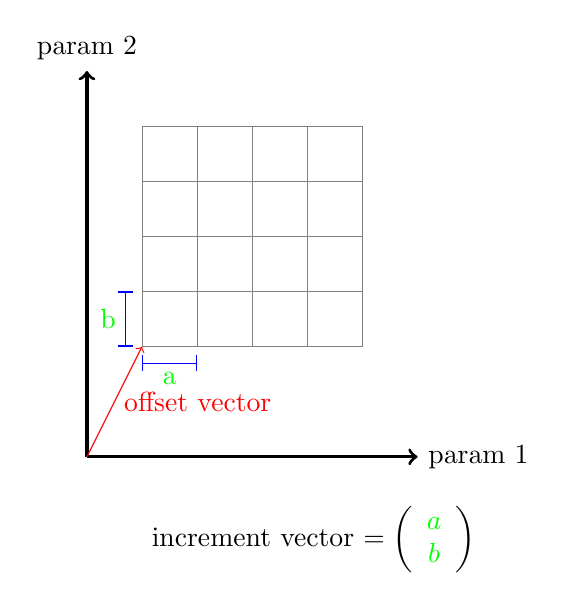
\begin{tikzpicture}[scale = 0.7]
		\draw[->, very thick] (0,0) -- (6, 0) node[right] {param 1};
		\draw[->, very thick] (0,0) -- (0, 7) node[above] {param 2};
		
		\draw[->, red] (0,0) -- node[right] {offset vector} (1, 2);
		
		\draw[step=1cm,gray,very thin] (1, 2) grid (5, 6);
		\draw[gray,very thin] (1, 2) -- (5, 2);
		\draw[gray,very thin] (1, 2) -- (1, 6);
		
		\draw (1, -1.5) node[right]{increment vector  $ = \left(\begin{array}{c} \textcolor{green}{a} \\ \textcolor{green}{b} \end{array}\right) \qquad$} ;
		
		 \draw[|-|, blue] (1, 1.7) -- node[below]{\textcolor{green}{a}} (2, 1.7);
		 \draw[|-|, blue] (0.7, 2) -- node[left]{\textcolor{green}{b}} (0.7, 3);
	\end{tikzpicture}
	\end{minipage}
\end{frame}

\begin{frame}
	\frametitle{Runtime Approximation I}
	\begin{minipage}[t]{0.40\linewidth}
		\begin{itemize}
			\item<2->{Determine the surrounding grid points to a task}
			%\item<2->{Calculate the influence factor $F_i$ per grid point}
			%\begin{itemize}
				%\item<3->{Check whether the distance to the point is 0}
				%\begin{itemize}
				%	\item<4->{ $\Rightarrow$ influence factor $F_i$ is 1 $($ 													$\widehat{=}$ 100$\%$ influence$)$}
				%\end{itemize}
				%\item<5->{Otherwise calculate $F_i$ $($'Kastrati' value $F_i$ for grid 										point i$)$}
				%\begin{itemize}
			%		\item<3->{$d_i = \frac{D_i}{\Sigma D_i}$ $\widehat{=}$ relative distance}
					%\item<4->{$d_i \widehat{=}$ relative distance to grid point i}
					%\item<7->{$D_i \widehat{=}$ absolute distance to grid point i}
					%\item<4->{$\Sigma D_i \widehat{=}$ total distance to all 													surrounding grid points}
			%\end{itemize}
			%		\item<4->{$F_i = \frac{1}{\frac{d_i}{d_0} + \frac{d_i}{d_1} + ... + 										\frac{d_i}{d_n}}$}
				%\end{itemize}
		\end{itemize}
	\end{minipage}\hfill
	\begin{minipage}[t]{0.60\linewidth}
	\vspace{-\ht\strutbox}
		\begin{tikzpicture}
	%\fill[white] (-2, 6) circle (0.01);
	
		\fill (1, 2) circle (0.5mm);
		\fill (5, 2) circle (0.5mm);
		\fill (1, 6) circle (0.5mm);
		\fill (5, 6) circle (0.5mm);
		
		\fill[green!75!black] (2, 2) circle (0.5mm) node[above]{$T_0$};
		\fill[green!75!black] (7, 3) circle (0.5mm) node[right]{$T_1$};
		\fill[green!75!black] (2, 5) circle (0.5mm) node[above]{$T_3$};
		\fill[green!75!black] (7, 4) circle (0.5mm) node[right]{$T_2$};
				
		\draw[->] (1, 2) -- (1.95, 2);
		\draw[->] (5, 2) -- (6.97, 2.97);
		\draw[->] (1, 6) -- (1.97, 5.03);
		\draw[->] (5, 6) -- (6.97, 4.03);		
		
		\fill[red] (5, 3) circle (0.5mm);
		
		\begin{scope}[>= Latex]
			\draw[->] (4, 3) node[left]{appearing task}  --  (4.95, 3) ;
		\end{scope}
	\end{tikzpicture}
	\end{minipage}\hfill
\end{frame}

\begin{frame}
	\frametitle{Runtime Approximation II}
	\begin{minipage}[t]{0.40\linewidth}
		\begin{itemize}
			%\item<1->{Determine the surrounding grid points to a task}
			\item<2->{Calculate the influence factor $F_i$ per grid point}
			%\begin{itemize}
				%\item<3->{Check whether the distance to the point is 0}
				%\begin{itemize}
				%	\item<4->{ $\Rightarrow$ influence factor $F_i$ is 1 $($ 													$\widehat{=}$ 100$\%$ influence$)$}
				%\end{itemize}
				%\item<5->{Otherwise calculate $F_i$ $($'Kastrati' value $F_i$ for grid 										point i$)$}
				%\begin{itemize}
					\item<3->{$d_i = \frac{D_i}{\Sigma D_i}$}
					%\item<4->{$d_i \widehat{=}$ relative distance to grid point i}
					%\item<7->{$D_i \widehat{=}$ absolute distance to grid point i}
					%\item<4->{$\Sigma D_i \widehat{=}$ total distance to all 													surrounding grid points}
			%\end{itemize}
					\item<4->{$F_i = \frac{1}{\frac{d_i}{d_0} + \frac{d_i}{d_1} + ... + 										\frac{d_i}{d_n}}$}
				%\end{itemize}
		\end{itemize}
	\end{minipage}\hfill
	\begin{minipage}[t]{0.60\linewidth}
	\vspace{-\ht\strutbox}
		\begin{tikzpicture}
	%\fill[white] (-2, 6) circle (0.01);
	
		\fill (1, 2) circle (0.5mm);
		\fill (5, 2) circle (0.5mm);
		\fill (1, 6) circle (0.5mm);
		\fill (5, 6) circle (0.5mm);
		
		\draw[->] (1, 2) -- (1.95, 2);
		\draw[->] (5, 2) -- (6.97, 2.97);
		\draw[->] (1, 6) -- (1.97, 5.03);
		\draw[->] (5, 6) -- (6.97, 4.03);
		
		%\fill[white] (1, 2) circle (0.5mm);
		%\fill[white] (5, 2) circle (0.5mm);
		%\fill[white] (1, 6) circle (0.5mm);
		%\fill[white] (5, 6) circle (0.5mm);
		
		\fill[green!75!black] (2, 2) circle (0.5mm) node[above]{$T_0$};
		\fill[green!75!black] (7, 3) circle (0.5mm) node[right]{$T_1$};
		\fill[green!75!black] (2, 5) circle (0.5mm) node[above]{$T_3$};
		\fill[green!75!black] (7, 4) circle (0.5mm) node[right]{$T_2$};
		
		\begin{scope}[>= Latex]
			\draw[<->, blue] (4.97, 2.99) -- node[below]{$D_0$} (2.03, 2.01);
			\draw[<->, blue] (5.05, 3) -- node[below]{$D_1$} (6.95, 3);
			\draw[<->, blue] (4.97, 3.02) -- node[above]{$D_3$} (2.03, 4.98);
			\draw[<->, blue] (5.02, 3.01) -- node[above]{$D_2$} (6.96, 3.98);
		\end{scope}
		
		\fill[red] (5, 3) circle (0.5mm);
	\end{tikzpicture}
	\end{minipage}\hfill
\end{frame}

\begin{frame}
	\frametitle {Runtime Approximation III}	
		\begin{itemize}
			\item<2->{The total sum of all influence factors is 1}
			\item<3->{Multiply the runtime of each grid point with its corresponding factor}
			\item<4->{Approximated runtime = $\sum t_i * F_i$}
			\item<5->{$t_i$ = runtime of grid point i}					
		\end{itemize}				
\end{frame}

\begin{frame}
	\frametitle{Task Insertion}
		\begin{itemize}
			\item<2->{Check whether the task is 'suited' as value of a 													surrounding grid point}
			\begin{itemize}
				\item<3->{grid points 'always' point to the closet task already inserted}
				\item<4->{note that inserting a point only adapts the 														closest grid points}
			\end{itemize}
			\item<5->{Adapt surrounding grid points, if necessary}
		\end{itemize}
		
		\begin{itemize}
			\item<6->{'Hard insert': check \textbf{all} grid points and eventually adapt them}
		\end{itemize}	
\end{frame}

\begin{frame}
	\frametitle{Evaluation}
		\begin{itemize}
			\item<2-> {Evaluation on each insert}
			\item<3-> {Calculate average deviation}
			\item<4-> {Compare with set threshold}
			\begin{itemize}
				\item<5->{deviation $>$ threshold: recreate grid}
			\end{itemize}
		\end{itemize}
\end{frame}	
	
\begin{frame}
	\frametitle{Creation}
		\begin{itemize}
			\item<2-> {Initialize offset vector}
			\begin{itemize}
				\item<3-> {first creation: 0}
				\item<4-> {later: smallest value}
			\end{itemize}
			\item<5-> {Initialize increment vector}
			\begin{itemize}
				\item<6->{first creation: 1}
				\item<7->{later: 'data size' divided by number of fields}
			\end{itemize}
			\item<8-> {'Hard Insert' all tasks stored in database}			
		\end{itemize}
\end{frame}

%										☺
%\begin{frame}
%	\frametitle{}
%\end{frame}
\section{GUI}
	\begin{frame}{Introduction}
		\begin{itemize}
			\pause
			\item The graphical user interface is an optional feature so the scientists can easily use MOAB Workload Manager and dynamic scheduler interface. 
			\pause
			\item The user can generate a shell script for MOAB Workload Manager and send it via SSH to the server.
			\pause
			\item User can also discover relationships in his/her tasks and observe the performance the program. 
			
		\end{itemize}
	\end{frame}
	
	\begin{frame}{Architecture}
		\begin{itemize}
			\item The main architecture pattern, the graphical user interface is oriented to, is the Model-View-
Presenter. 
	        \item The view of the user interface is developed in the FXML scripting language and Java code is used for application logic.
	        
				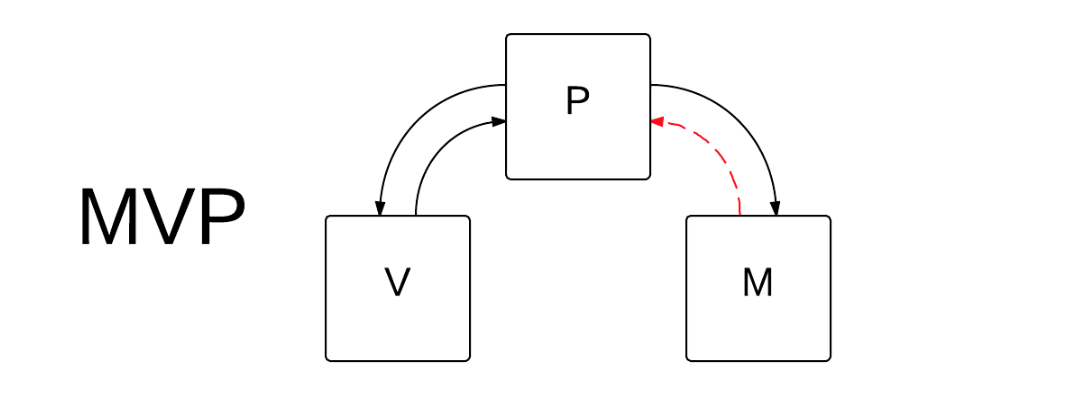
\includegraphics[width=300px, height=100px]{images/mvp.png}
		\end{itemize}
	\end{frame}
%	\subsection{Design}
	\begin{frame}{Architecture (Design)}
		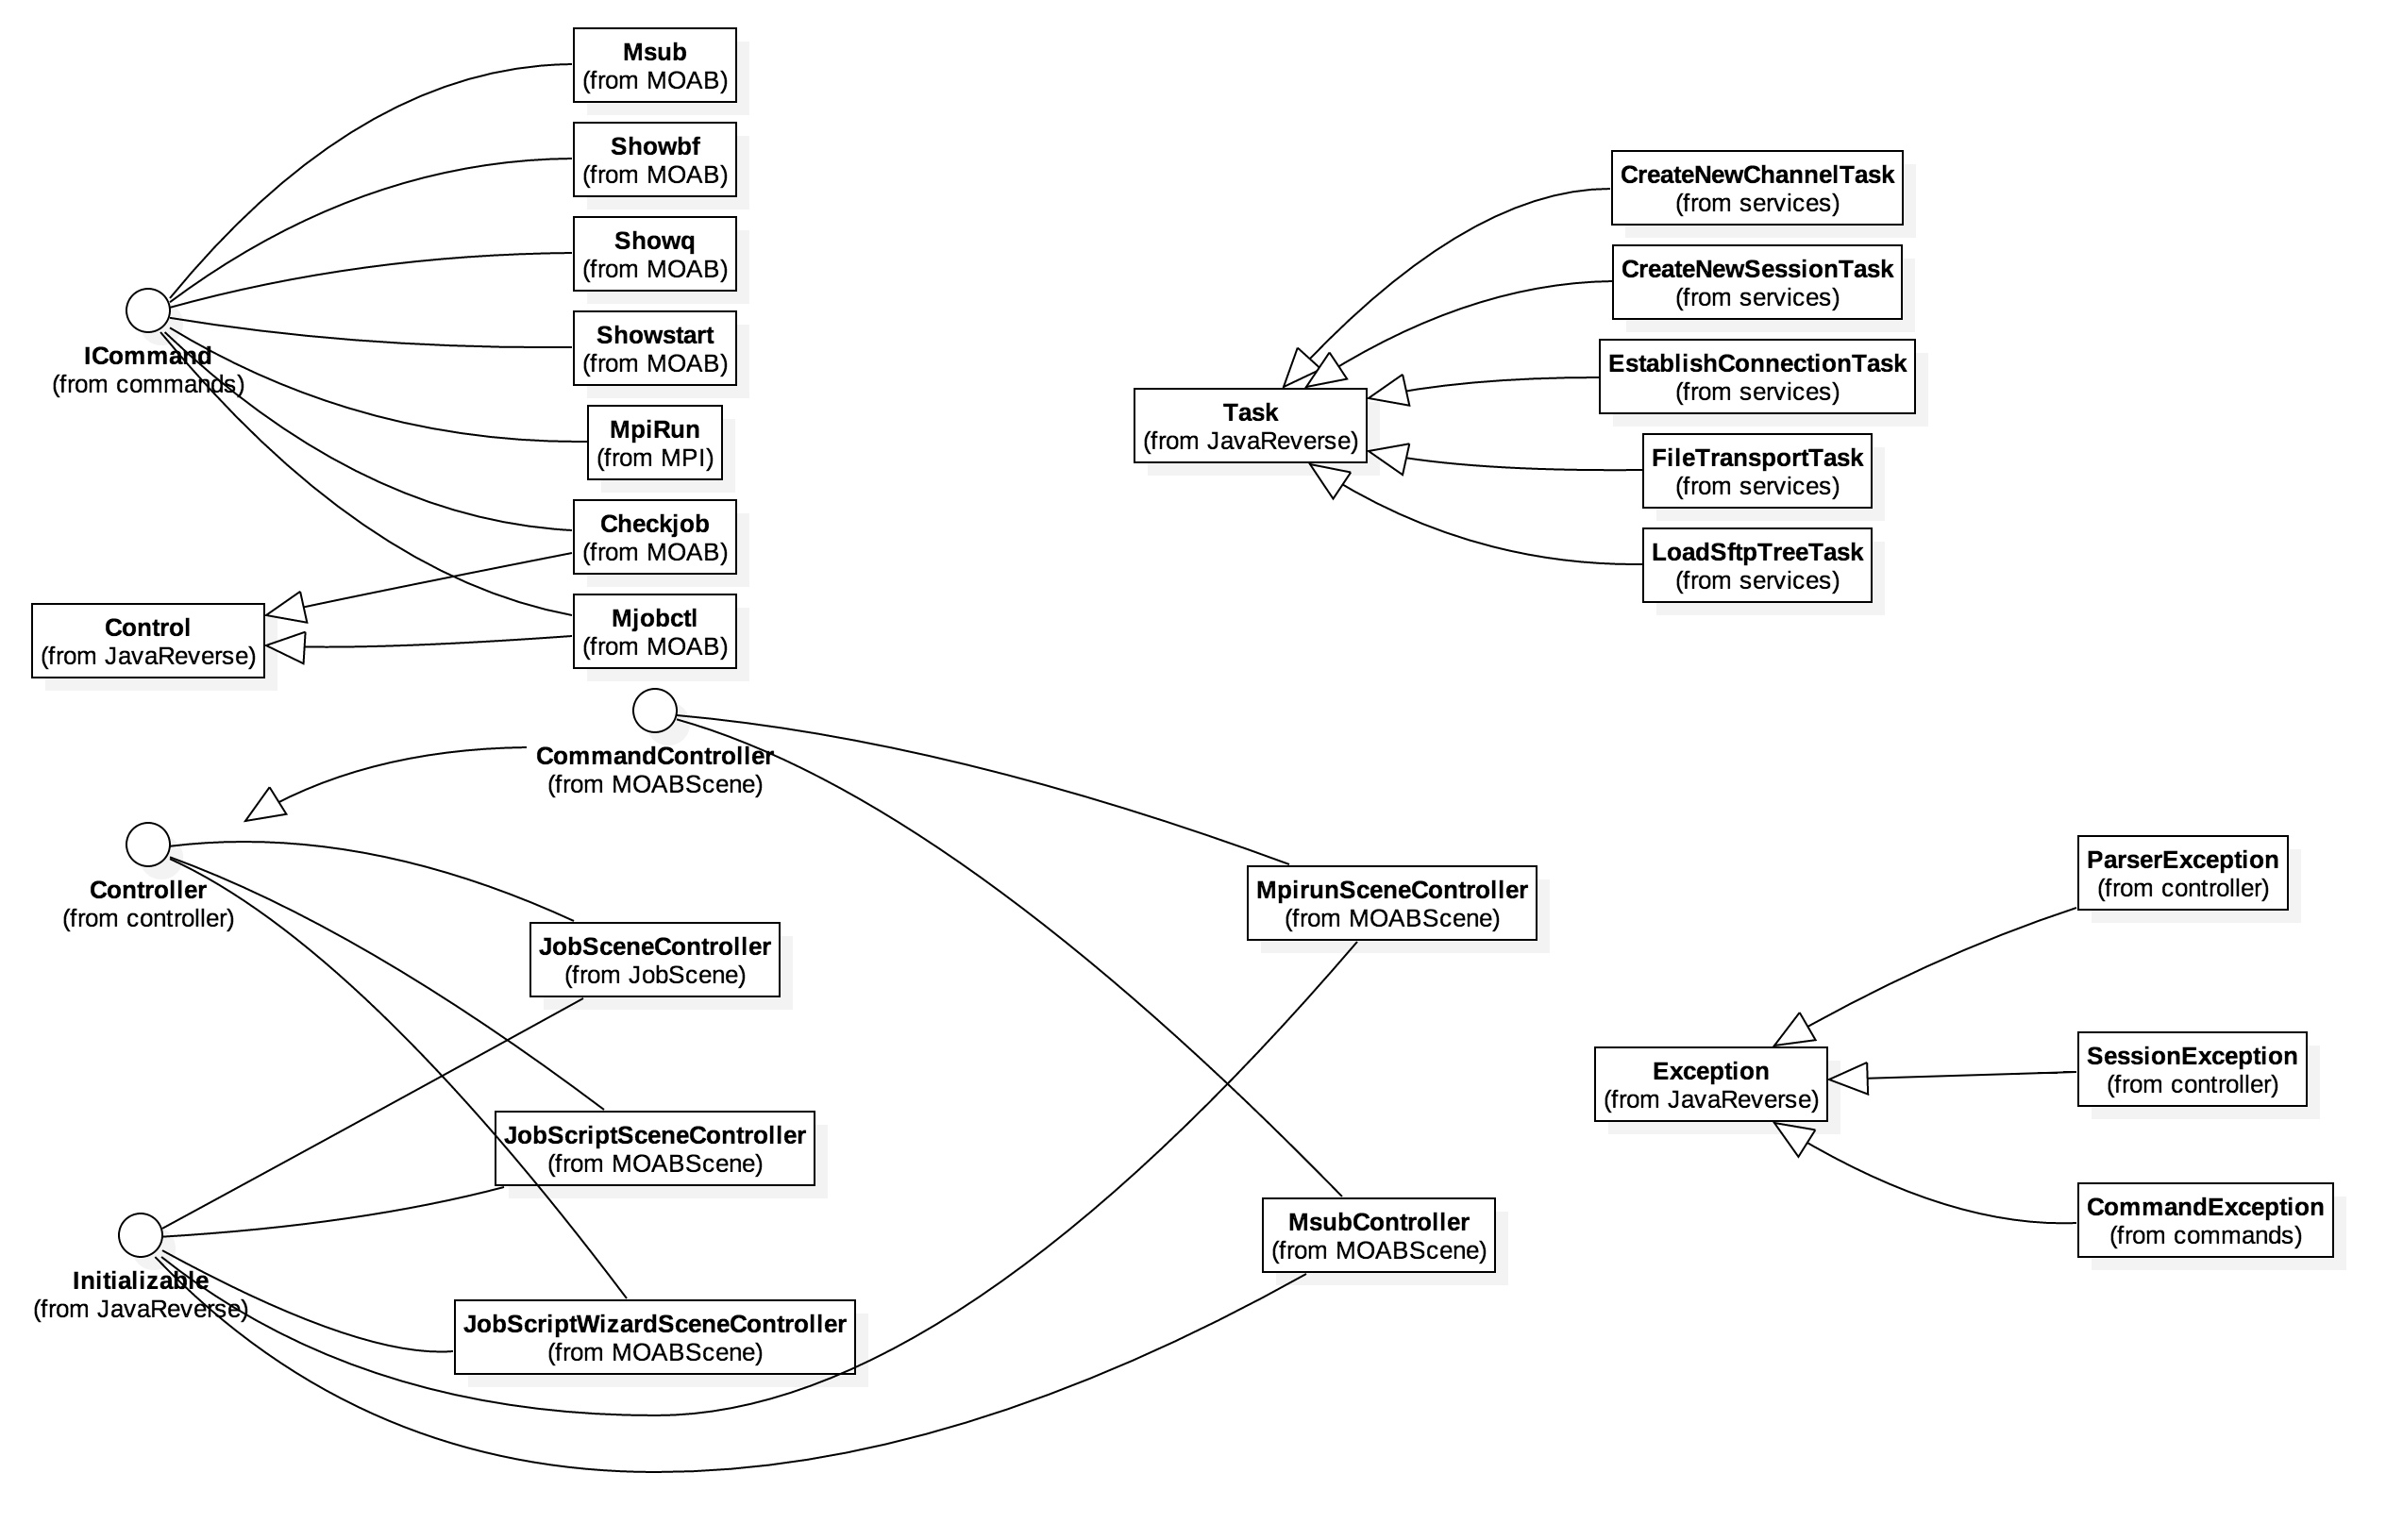
\includegraphics[width=300px, height=210px]{images/GUIDesign.png}
	\end{frame}
	

	\begin{frame}{SSH-Connection}
		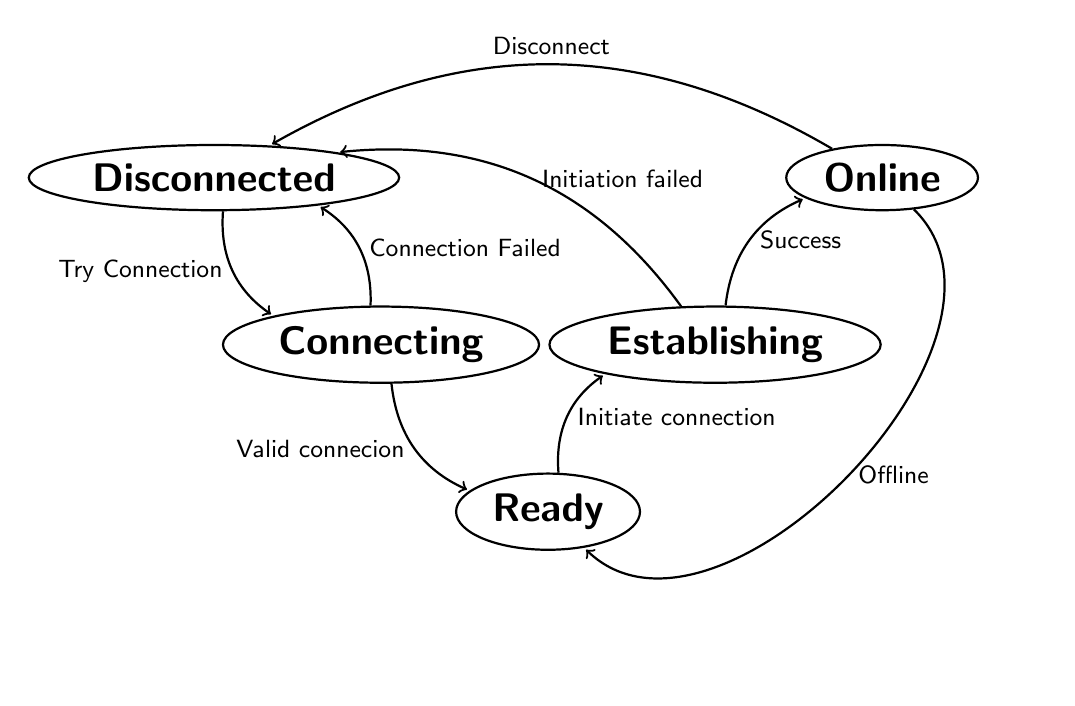
\begin{tikzpicture}[->,shorten >=1pt,auto,node distance=3cm,thick,main node/.style={ ellipse,draw,font=\sffamily\Large\bfseries}]
 
  \node[main node] (1) {Disconnected};
  \node[main node] (2) [below right of=1]{Connecting};
  \node[main node] (3) [below right of=2] {Ready};
  \node[main node] (4) [above right of=3] {Establishing};
  \node[main node] (5) [above right of=4] {Online};

  \path[every node/.style={font=\sffamily\small}]
    (1) edge [bend right] node[left] {Try Connection} (2)
        
    (2) edge [bend right] node[right] {Connection Failed} (1)
        edge [bend right] node[left] {Valid connecion} (3)
    (3) edge [bend left] node[right] {Initiate connection} (4)
    		
    (4) edge [bend right] node[right] {Initiation failed} (1)
       	edge [bend left] node[right] {Success} (5)
    (5)  edge [bend right] node[above] {Disconnect} (1)
         edge [bend left=90] node[right] {Offline} (3);
	\end{tikzpicture}
	\end{frame}
	
	\begin{frame}{Script generator}
		Shell script generator for MOAB Workload Manager :
		
		\begin{itemize}
			\pause
			\item Parses msub command
			
			\pause			
			\item Specifies the directory in server using lazy tree 
			 
			\pause
			\item Parses mpirun command
			
			\pause
			\item Parses parameters of the dynamic scheduler
		\end{itemize}
	\end{frame}
	
	
	
	\begin{frame}{Script generator (Structure)}
		
		\begin{block}{run\_scheduler.sh}
		        \#\#\#\# MOAB commands
		        \newline
		        \newline
				\#MSUB  -q develop\\
				\#MSUB  -l nodes=22:ppn=22\\
				\#MSUB  -l walltime=1000\\
				\#MSUB  -M uxdok@student.kit.edu
				\newline
				\newline
        				\#\#\#\# Directory
				\newline
				\newline
				cd ./Documents
				\newline
				\newline
        				\#\#\#\# MPI commands
        			\newline
        			\newline
				mpirun -np 4 ./myExec -design master-worker -strategy fifo
			
		\end{block}
	\end{frame}
\begin{frame}
	\begin{center}
			\huge{\textbf{Live Demo}}
	\end{center}		
\end{frame}
\section{Statistics}
\begin{frame}{Statistics}
	\begin{itemize}
		\item approx. 300 commits during 143 days
		\item average 2.1 commits per day
		\item 4000 lines of Java code
		\item 3500 lines of C++ / C code
		\item TeX, Makefile and XML
	\end{itemize}
\end{frame}

\begin{frame}{Experience}
	\begin{itemize}
		\item it is hard to understand what is the actual problem
		\item bigger changes during the implementation are hard to handle
		\item how fast you can learn a unknown language (C++)
	\end{itemize}
\end{frame}
\begin{frame}
	\begin{center}
			\huge{\textbf{End}}
	\end{center}		
\end{frame}
\end{document}
